\subsection{Descripción del problema.}

\vspace*{0.3cm}

Dado un \textbf{tablero de ajedrez de tamaño $n$x$n$ y $k$ caballos ocupando
inicialmente ciertos casilleros (aleatorios)} del mismo, el objetivo consiste
en \textbf{reunir a todos los caballos en un mismo casillero, minimizando la
cantidad total de movimientos realizados}. Esta cantidad equivale a
\textbf{la suma de los movimientos de todos los caballos} en el tablero.

Un caballo $k$ puede moverse únicamente \textbf{respetando los movimientos
válidos según las reglas del ajedrez}. Además, \textbf{un casillero puede
estar ocupado por más de un caballo simultáneamente}.

\vspace*{0.5cm}

\textbf{Ejemplo:}

En un tablero de 8x8, con 3 caballos en las posiciones [2,2], [5,5] y [2,8],
la menor cantidad de saltos posibles es 4, haciendo que los caballos de los
extremos cayan hacia la posición del caballo del medio[5,5], como se puede ver
en la siguiente imagen:

\begin{figure}[htb]
  \begin{center}
      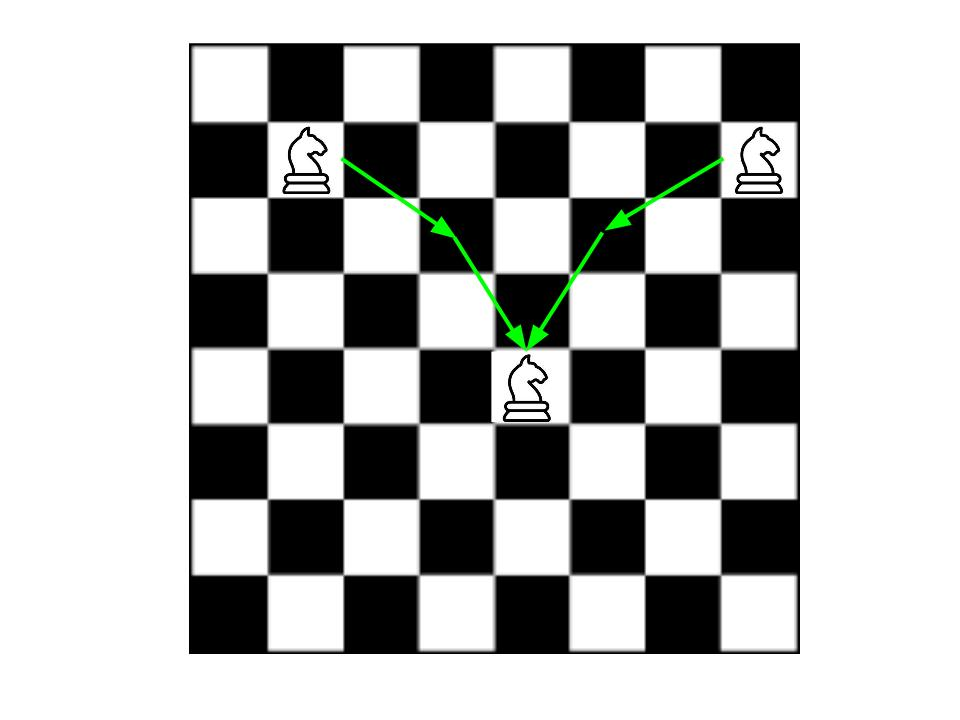
\includegraphics[scale=0.25]{imagenes/caballos.jpg}
  \end{center}
  \caption{ejemplo de tablero.}
\end{figure}


\newpage
\subsection{Desarrollo de la idea y pseudocódigo.}

\vspace*{0.3cm}


Para resolver este problema, utilizaremos $k$ tableros de $n$x$n$ casilleros,
uno por cada caballo. En cada tablero se calculará el costo para dicho caballo
de llegar a cada casillero, aplicando \textit{BFS} desde el casillero inicial,
quedando inválidos los casilleros que no pueden alcanzarse.

Luego se recorren todos los casilleros, sumando el valor de éstos en todos los
tableros (si son alcanzables), obteniendo así el costo de cada casillero para
cada caballo. De existir, el mínimo de estos valores será el casillero que
pueden alcanzar todos los caballos en la menor cantidad de saltos.

%\begin{codebox}
%\Procname{$\proc{puntoDeEncuentro}(caballos, n)$}
%\li $\id{tableros} \gets \emptyset$
%\li \For $caballo \in caballos$
%\li   \Do
%\li       $\proc{agregar}(\proc{crearTablero}(caballo,n), tableros)$
%      \End
%\li $\id{i} \gets 0$
%\li $\id{j} \gets 0$
%    $\id{min_i} \gets -1$
%    $\id{min_j} \gets -1$
%    $\id{min} \gets -1$
% \li \While $\id{i} < \id{n}$
% \li   \Do
% \li     \While $\id{j} < \id{n}$
% \li       \Do
% \li         $\id{sum} \gets 0$
% \li         $\id{caballo} \gets 0$
% \li         \While $\id{caballo} < \proc{tamaño}(caballos)$
% \li           \Do
%                 if (tableros[caballo][i][j] == -1)
%                   sum = -1
%                 else if (sum != -1)
%                   sum += tableros[caballo][i][j]
%                 end
%                 caballo++
%               \End
%             if (sum != -1 && (min == -1 || sum < min))
%               min = sum
%               min_i = i
%               min_j = j
%             end
%             j++
%         \End
%         i++
%       \End
%     if min == -1
%       \Return 'no'
%     else
% \li \Return min min_i min_j
% \end{codebox}
%
%
% crearTablero



\newpage
\subsection{Justificación de la resolución y demostración de correctitud.}

\vspace*{0.3cm}

La solución es el mínimo número de movimientos entre todos los caballos que
los deja en el mismo casillero.

Primero completamos cuanto le cuesta a cada caballo llegar a cada
casillero, para calcular esto tomamos al tablero como un grafo, cada
casillero como un nodo y los ejes los posibles saltos de caballo. Empezando
desde la posición del caballo, se recorre de una forma Breadth-First,
logrando de esta manera poner la cantidad mínima de saltos para cada
casillero alcanzable, ya que el algoritmo BFS obtiene todos los caminos
mínimos desde un nodo inicial.

Luego, simplemente es cuestión de obtener el mínimo de la sumatoria para cada casillero.
Recorremos todos los casilleros para cada tablero (de cada caballo),
tomando el valor mínimo (únicamente si es posible llegar a ese casillero
con todos los caballos).
Este mínimo (si existe) es una solución óptima.

\newpage
\subsection{Análisis de complejidad.}

\vspace*{0.3cm}

\textcolor{red}{\textbf{completar!}}
Para el análisis de complejidad nos basaremos en el pseudocódigo de la función
\textsc{puntoDeEncuentro}, correspondiente al ítem \textbf 4.2

\begin{enumerate}

 \item \textbf{Aclaraciones} : Se considerará $k$ = cantidad de caballos
 y $n$ = cantidad de casilleros de alto o largo (es indiferente ya que los
 tableros serán cuadrados).

 \item Las operaciones sobre el contenedor \verb|vector| de la STL (push_back, 
 begin y end) y la creación de sus iteradores toman $O(1)$.
 
 \item En la función \verb|main| la estructura \verb|for| es ejecutada
  $k$ veces, donde se realiza un \verb|make_pair| y un \verb|push_back| 
  sobre un \verb|vector| que cuestan $O(1)$, dando una complejidad de $O(k)$.
   
 \item Crear la esctructura \verb|pair| $respuesta $que contrendrá el 
 resultado del problema, si lo hay, cuesta $O(1)$.
 
 \item En la función \verb|punto_de_encuentro| se crea el \verb|vector| 
 $tableros$ ( $O(1)$ ), y con un iterador se recorre el \verb|vector| $caballos$ en 
 $O(k)$ donde por cada iteración se crea un tablero (ver \textbf{Tablero}) 
 ( $O(n^{2})$ ), se crea un \verb|queue| para los casilleros ( $O(1)$ ), 
 se crea un \verb|make_pair| ( $O(1)$ ) y se los inserta en el \verb|queue| $casilleros$
 mediante \verb|push| ($ O(1)$ ), se llena el tablero creado (ver \textbf{LLenar tablero}) 
 en $O(n^{2})$ y se los agrega a $tableros$ con \verb|push_back| en $O(1)$
  dando una complejidad total de $O(k.(n^{2} + n^{2}))$ = $O(k.n^{2})$.
 
 \item \textbf{Tablero} - Crear un tablero implica crear un \verb|vector| 
 que contendrá otro \verb|vector| dentro ($O(1)$) y se le dará tamaño $n$
 al vector contenedor con \verb|resize| en $O(n)$. Luego se creará un iterador
 ($O(1)$) para recorrer el \verb|vector| contenedor ($O(n)$) y en cada iteración
 al \verb|vector| contenido en dicha posición se le seteará $n$ posiciones
 en $-1$, dando una complejidad total de $O(n^{2})$.
 
 \item \textbf{Llenar tablero} - La función posee un \verb|while| donde se ejecutan
 todas las instrucciones, mientras el \verb|queue| $casilleros$ sea diferente de vacío.
 $casilleros$ comienza con 1 elemento y en cada ejecución se le realiza
 \verb|pop| de un elemento y se le agregan todas las posiciones a las cuales se 
 pueden saltar (siguendo el patron del caballo y sin que salga del tablero), la 
 complejidad del \verb|while| sera de $O(n^{2})$ en el peor caso (todos los casilleros), multiplicado 
 por la complejidad de las instrucciones que se ejecuten dentro del mismo.
 
 Crear un \verb|pair| y asignarle el \verb|first| de la tupla del primer elemento 
 de $casilleros$ cuesta $O(1)$, al igual que crear un \verb|int| y asignarle el
 \verb|second| de la tupla del primer elemento de $casilleros$.
 
 Hacer \verb|pop| de $casilleros$ cuesta $O(1)$.
 
 En el primer \verb|if| acceder al elemento $[x][y]$ del \verb|vector[vector]| 
 $t.casilleros$ del tablero y compararlo con -1 cuesta $O(1)$ (notar que $tablero$ 
 posee un $casilleros$ \verb|vector[vector]| y que la función recibe otro $casilleros$ 
 \verb|queue|). En caso de ser verdadero se realiza un \verb|continue| en $O(1)$.
 
 Asignarle al \verb|int| $nivel$ un elemento de $t.casilleros$ en $[x][y]$ cuesta $O(1)$.
 
 Para las ocho posiciones posibles a las que puede saltar un caballo desde la posición
 actual, validar que la posición sea válida (que caiga dentro del tablero) cuesta 
 $O(1)$, y de ser válida ver si el valor almacenado en dicho lugar es distinto de -1
 también cuesta $O(1)$. Si se cumplen estas condiciones se ejecuta la instrucción 
 del if donde se agrega el casillero que se acaba de evaluar al \verb|queue| $casilleros$
 ($O(1)$) que se recorre en el \verb|while|, realizando dos \verb|make_pair| ($O(1)$) 
 y asignandole el valor del $nivel$ + 1 ($O(1)$).
 
\end{enumerate}

\newpage
\subsection{Experimentación y gráficos.}

\vspace*{0.3cm}

\subsubsection{Test 1 - benchmark caso aleatorio}

\textcolor{red}{\textbf{completar!}}


\newpage
\subsubsection{Test 2 - benchmark del peor caso}

Este ejercicio no tiene mejor y peor caso, todos tardan lo mismo.
Porque en todos los casos se generan los tableros para todos los caballos
y también se busca el mínimo en todos los casilleros.-
\textcolor{red}{\textbf{completar!}}


\newpage
\subsubsection{Test 3 - benchmark del mejor caso}

\textcolor{red}{\textbf{completar!}}
